% Report of the SS16 - X-ray Diffraction mini-project
% By Lyubomir Shoylev, 2022.
\documentclass[11pt,a4paper,twoside,onecolumn]{article}
\title{\textbf{SS16: X-ray diffraction and X-ray spectroscopy (mini-project)}}
\author{Lyubomir Shoylev, shil5377}
\date{\today}
% My report package :)
\usepackage{my-report}
\usepackage[default-range=1-1]{lipsum}
\newcommand{\reminder}[1]{\textcolor{red}{#1}}
\newcommand{\rydberg}{R}
\newcommand{\Kalpha}{$\mathrm{K}_\alpha$~}
\newcommand{\Kbeta}{$\mathrm{K}_\beta$~}
\newcommand{\Lalpha}{$\mathrm{L}_\alpha$~}

\begin{document}
\maketitle

\begin{abstract}
    In this experiment, we study the production of X-ray emission lines and verify Moseley's Law by measuring the energy of emission line series in several metals. Then, we use spectroscopy to report on the composition of different samples: two semiconductors, several unlabelled alloys and international metal coins. We give results for the mass ratios of the unlabelled alloys. We also find that most coins are made up of either Ni-Cu or Cu-Zn alloys and expand on the reasons behind this choice.
\end{abstract}

\section{Introduction}
X-rays are an important experimental tool and have been for more than a 100 years, ever since their discovery by Wilhelm R\"{o}ntgen. They are currently employed by both scientists, from scattering experiments in condensed matter to high-energy astrophysics, and citizens for various medical purposes and security scanners. In this experiment, we first study the theoretical basis of X-ray production, first developed by Moseley. We measure the energy of the \Kalpha and \Lalpha emission line series of several samples of known elements with known atomic number, $Z$, to verify Moseley's Law. Having established the uniqueness of X-ray emission lines for a given $Z$, we use it to study the composition of several samples provided to us in the laboratory by measuring their emission spectra when exposed to a continuous X-ray source. We begin by independently confirming the composition of two semiconductor samples observed in the non-mini-project part of the experiment \reminder{--- remove this and fix non-MP part}. Then we report on the composition of several unlabelled metal alloys and the relative mass ratios of the samples. Finally, we report on the composition of an array of international coins and expand more on the reasoning for the mainly Ni-Cu-Zn composition.

\section{Theory}
We begin by introducing some of the background theory behind X-rays and their production.
\subsection{X-ray atomic spectra}
The emission spectra of atoms is due to energy transitions of shell electrons from a higher- to a lower-energy level. We are interested in X-rays, specifically, which are due to transitions in the inner electron levels of high-$Z$ atoms. These are shielded from the outer electron layers and are mostly unaffected by the chemical structure of the sample i.e. by the surrounding atoms. Therefore, we can take an energy level of an electron to be $E_n = -\rydberg\left(Z\right) / n^2$ where $\rydberg \left(Z\right)= \rydberg_\infty \left(Z - b\right)^2$ is the modified Rydberg constant for a given $Z$, $b$ is an atom-dependent parameter, and $\rydberg_\infty$ is the hydrogen Rydberg constant. Then, the energy of an emitted photon by a transition from level $n_\mathrm{i}$ to $n_\mathrm{f}$ is given by:
\begin{equation}\label{eqn:x-ray-energy}
    \varepsilon = \rydberg\left(Z\right) \left(\frac{1}{n_\mathrm{f}^2} - \frac{1}{n_\mathrm{i}^2}\right).
\end{equation}
We can rewrite this at fixed $n_\mathrm{i}$, $n_\mathrm{f}$ (i.e. for a given line) as:
\begin{equation}\label{eqn:moseleys-eqn}
    \sqrt{\varepsilon} = m \times Z + C,
\end{equation}  where $m$, $C$ are constants. This relationship is known as `Moseley's Law'.

The name convention of the low-$n$ energy levels in X-ray notation is given in Table \ref{tab:siegbahn-notation}. The energy difference between different L, M levels is not large, so if we have a low resolution detector we usually observe e.g. only one \Kalpha line.\reminder{quantify this plox.}
\begin{table}[!htbp]
    \centering
    \begin{tabular}{@{}llll@{}}
    \toprule
    \multicolumn{1}{c}{Initial level} & \multicolumn{1}{c}{Final level} & \multicolumn{1}{c}{Siegbahn notation} & \multicolumn{1}{c}{IUPAC notation} \\ \midrule
    \multirow{4}{*}{K ($1\mathrm{s}_{1/2}$)}  & L3 ($2\mathrm{p}_{3/2}$) & $\mathrm{K}_{\alpha 1}$ & K-L3  \\
                                              & L2 ($2\mathrm{p}_{1/2}$) & $\mathrm{K}_{\alpha 2}$ & K-L2  \\
                                              & M3 ($3\mathrm{p}_{3/2}$) & $\mathrm{K}_{\beta 1}$  & K-M3  \\
                                              & M2 ($3\mathrm{p}_{1/2}$) & $\mathrm{K}_{\beta 3}$  & K-M2  \\
    \multirow{2}{*}{L3 ($2\mathrm{p}_{3/2}$)} & M5 ($3\mathrm{d}_{5/2}$) & $\mathrm{L}_{\alpha 1}$ & L3-M5 \\
                                              & M4 ($3\mathrm{d}_{3/2}$) & $\mathrm{L}_{\alpha 2}$ & L3-M4 \\
    L2 ($2\mathrm{p}_{1/2}$)                  & M4 ($3\mathrm{d}_{3/2}$) & $\mathrm{L}_{\beta 1}$  & L2-M4 \\
    M5 ($3\mathrm{d}_{5/2}$)                  & N7 ($4\mathrm{f}_{7/2}$) & $\mathrm{M}_{\alpha 1}$ & M5-N7 \\ \bottomrule
    \end{tabular}
    \caption{Table of the connection between Siegbahn and IUPAC notation. Energy levels in IUPAC are listed with atomic notation as well. Source: \cite{Jenkins1991}.}
    \label{tab:siegbahn-notation}
\end{table}

\subsection{X-ray production}\label{subsec:x-ray-production}
In practice, we produce X-rays by bombarding a sample of some material with high energy electrons or X-rays which removes one of the inner shell electrons from the sample atom. This produces a vacancy in the shell. The vacancy is filled by an electron of a higher-$n$ orbit (see Figure \ref{fig:emission-diagram}), and the fall of potential energy of the electron is compensated by an emitted X-ray (ignoring higher order effects like the \emph{Auger effect}).

\begin{figure}[!htbp]
    \centering
    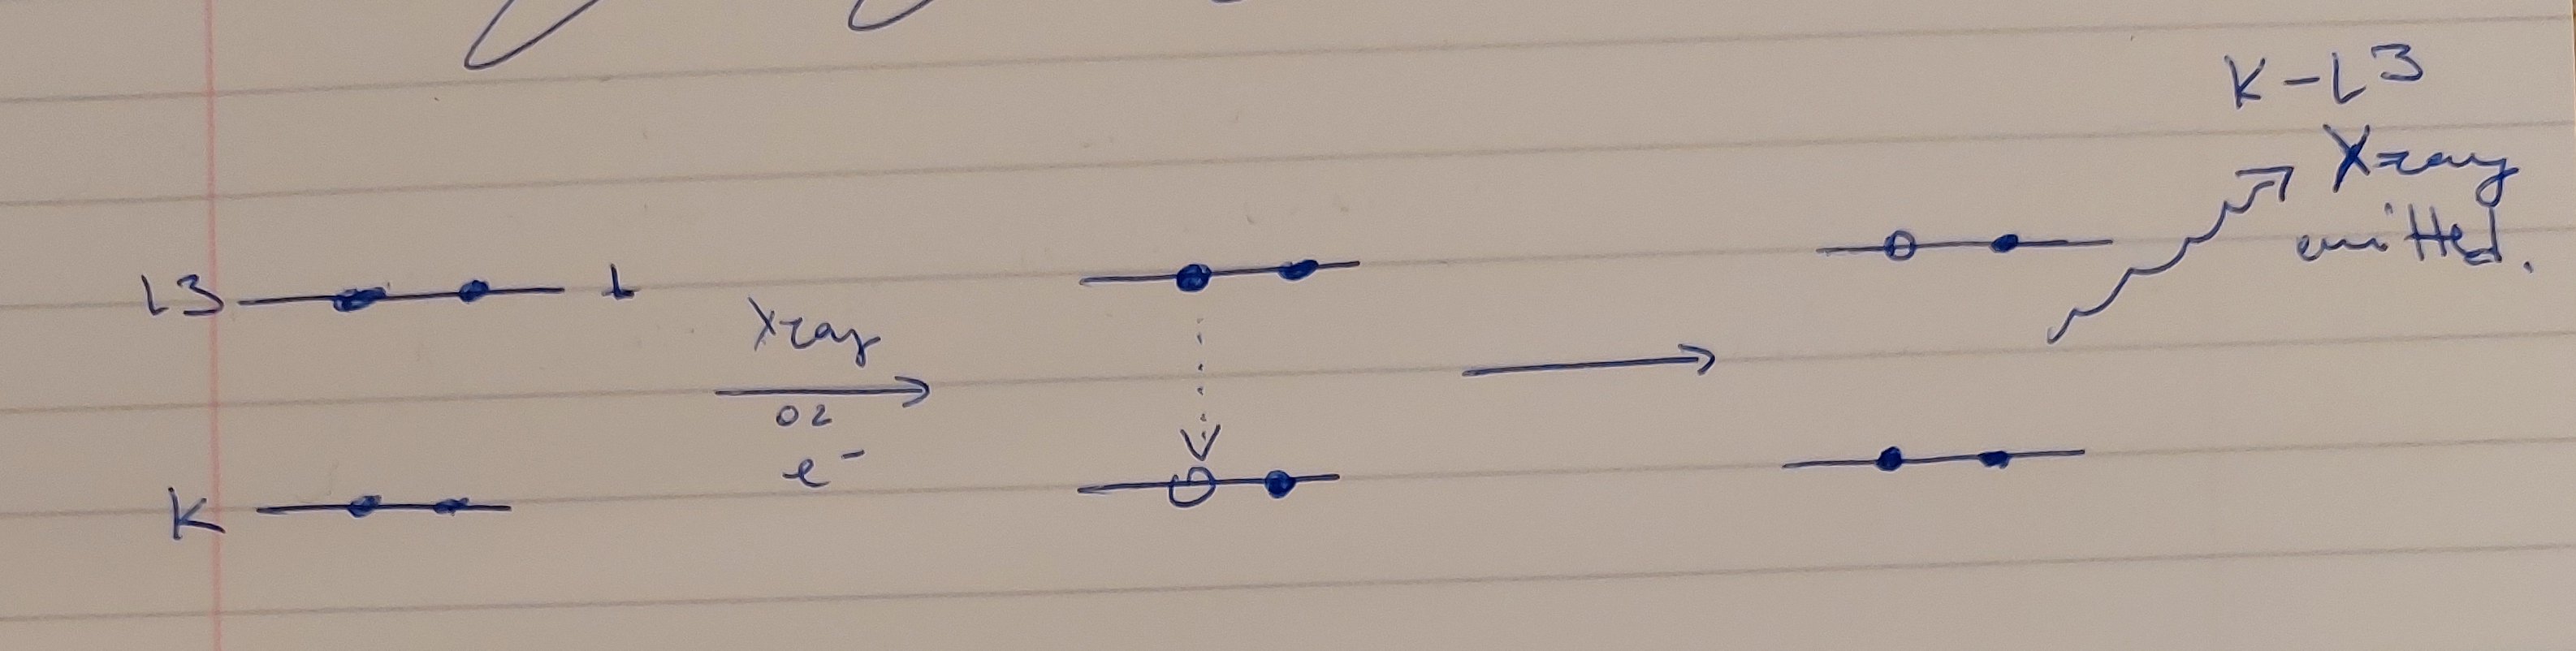
\includegraphics[width=\textwidth]{img/emission-diagram.png}
    \caption{Schematic of the emission process for a K-L3 transition.}\label{fig:emission-diagram}
\end{figure}

Usually, small laboratory X-ray tubes use an electron source. Because of that, we observe a continuum of X-ray radiation imposed on top of the emission lines. This radiation is called \emph{bremsstrahlung} (``braking") radiation. Its source is the interaction between decelerating electrons and stationary charges in the sample lattice. The maximal energy of a bremsstrahlung continuum is limited by the energy of the decelerating particle. If these are electrons accelerated by a potential difference $V$, then the maximal energy is given by: 
\begin{equation}\label{eqn:bremss-energy-max}
    \varepsilon_\mathrm{max} = eV.
\end{equation}

Suppose we use one such continuous X-ray source for the production of X-rays from a sample. We will take the K-series as an example. To produce a vacancy, an X-ray of energy $\varepsilon_\mathrm{in} = - E_1 = \rydberg(Z)$ is needed, which will be provided by a collision with an electron with maximum energy $\varepsilon_\mathrm{max}$ in the case of the X-ray source. The resultant energy of the emitted X-ray will be given by Equation \eqref{eqn:x-ray-energy}. Take, for example, the K-L transition: its energy will therefore be (ignoring fine-structure):
\begin{equation}\label{eqn:Kalpha-energy-out}
    \varepsilon_\mathrm{out} = \rydberg\left(Z\right) \left(1 - \frac{1}{2^2}\right).
\end{equation}
A process like this, in which $\varepsilon_\mathrm{in} \neq \varepsilon_\mathrm{out}$, is called \emph{fluorescence}.

\subsection{Composition analysis}\label{subsec:compos-analysis}
As previously stated, the X-ray emission is relatively independent of the composition of the sample. We can use this fact to perform a composition analysis on a sample by exposing it to the continuous bremsstrahlung of a source; this will allow the different components to fluoresce. The signal will give us information not only on \emph{which} elements are present (given that the source is high enough to allow fluorescence), but their relative contribution --- the intensity of the signal will depend only on the number density, $n$. Suppose we measure the intensity of a two-metal alloy with the peaks in the \Kalpha line as $I_\mathrm{a}$ and $I_\mathrm{b}$.
This tells us that:
\begin{equation}
    \frac{I_\mathrm{a}}{I_\mathrm{b}} = \frac{n_\mathrm{a}}{n_\mathrm{b}},
\end{equation}
where $n_\mathrm{a}$ and $n_\mathrm{b}$ are the number densities of materials a and b. From that, we could easily calculate percentage compositions for number densities or mass densities:
\begin{equation}
    \rho = n \times \mu, \quad \mu = \text{molar mass}.
\end{equation}

\section{Experiment}\label{sec:experiment}
Our experiment consists of the setup presented in Figure \ref{fig:experim-setup}. First, we have an X-ray source with a molybdenum anode, which produces some characteristic \Kalpha X-rays that can be used for diffraction experiments (see the first part of \cite{OxfPhys2010} \reminder{fix this plox}) and some continuous bremsstrahlung (see Section \ref{subsec:x-ray-production} for more details). These X-rays are focused through a circular aperture towards a target sample. The incident X-rays excite inner shell electrons, and the targets emit mostly in the characteristic X-rays of K, L, and M series. We detect these via an energy spectrometer that is sensitive in the region of our experiment. The setup parameters are: tube voltage $V = \qty{35}{kV}$, emission current \qty{1}{A}, exposure time $t=\qty{100}{s}$. This, according to Equations \eqref{eqn:bremss-energy-max} and \eqref{eqn:Kalpha-energy-out}, allows us to produce, for example, \Kalpha X-rays with energy up to \qty{26.25}{keV} from samples with atomic numbers up to at least $50$, ignoring the contribution from $b$.

\begin{figure}[!htbp]
    \centering
    \includegraphics[width=\textwidth]{img/experim-setup.png}
    \caption{Diagram of the experimental setup. More information can be found in the text of Section \ref{sec:experiment}.}\label{fig:experim-setup}
\end{figure}

To operate the apparatus and extract data, we use the software \emph{CASSY Lab 2} (see \cite{cassylab2}). The program has a built in database for the X-ray emission lines of most elements. It also allows for calculating a peak centre and fitting Gaussian profiles with specified energy to find the intensity of emission lines. (\reminder{expand on applicability since x-ray lines are asymmetrical.})

Before determining the energies, we first need to calibrate the energy scale. We will use two known samples - Fe and Ag. We choose these two samples since their \Kalpha lines lie at the two ends of the range of energies for which our samples have emission lines. The particular lines which we use to calibrate are the Fe \Kalpha with $E_\mathrm{Fe} = \qty{6.40}{keV}$ and the Ag \Kalpha with $E_\mathrm{Ag} = \qty{22.17}{keV}$. Also note the observational lower and upper limits, respectively \qtyrange{2}{4}{keV} and $\approx \qty{35}{keV}$. The calibration spectra are presented in Figure \ref{fig:calibration}.

\begin{figure}[!htbp]
    \centering
    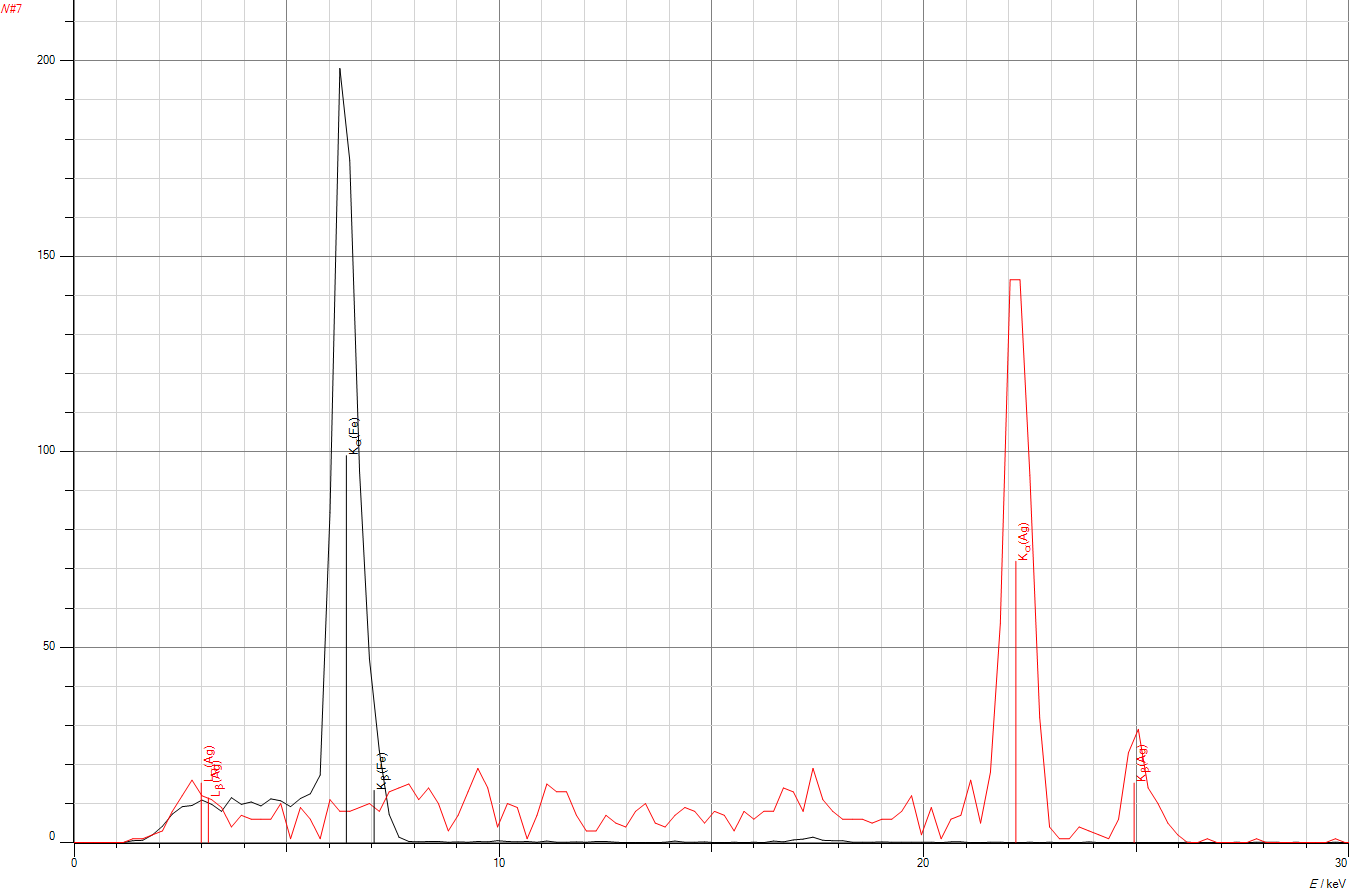
\includegraphics[width=0.5\textwidth]{img/calib.png}
    \caption{Fe and Ag spectra used for calibration. On the x-axis, we have the energy of the detected signal in \unit{keV}. On the y-axis, we have the signal counts for the Ag spectrum. \reminder{fix figure}}\label{fig:calibration}
\end{figure}

The first part of the experiment will test the validity of Moseley's Law making use of several samples of known substances.

The second part and third part of the experiment will utilise our knowledge about X-rays to learn more about the composition of other samples, and about some metal coins from around the world.

\section{Result and Analysis}

\subsection{Moseley's Law}
We measure the line energy values from the labelled samples. We can separate these in two groups:
\begin{itemize}[noitemsep]
    \item those whose \Kalpha lines lie in the observable range (excluding our two calibration points);
    \item those whose \Lalpha lines lie in the observable range.
\end{itemize}
Recalling Equations \eqref{eqn:x-ray-energy} and \eqref{eqn:moseleys-eqn}, we expect to fit the data for the two groups with a straight line for each group. The slope $m$ depends purely on the line we are observing, i.e. on the $n_\mathrm{i}, n_\mathrm{f}$ for the given line. We can predict the ratio of the constants for the two series. Following Equations \eqref{eqn:x-ray-energy} and \eqref{eqn:moseleys-eqn}, we get:
\begin{equation}
    m_\mathrm{K} = \sqrt{\rydberg_\infty} \left(1 - \frac{1}{2^2}\right)^{\sfrac{1}{2}} \propto \sqrt{\frac{3}{4}},\quad m_\mathrm{L} = \sqrt{\rydberg_\infty} \left(\frac{1}{2^2} - \frac{1}{3^2}\right)^{\sfrac{1}{2}} \propto \sqrt{\frac{5}{36}} \quad \Rightarrow \quad \frac{m_\mathrm{K}}{m_\mathrm{L}} = \sqrt{\frac{27}{5}}.
\end{equation}

\begin{figure}[!htbp]
    \centering
    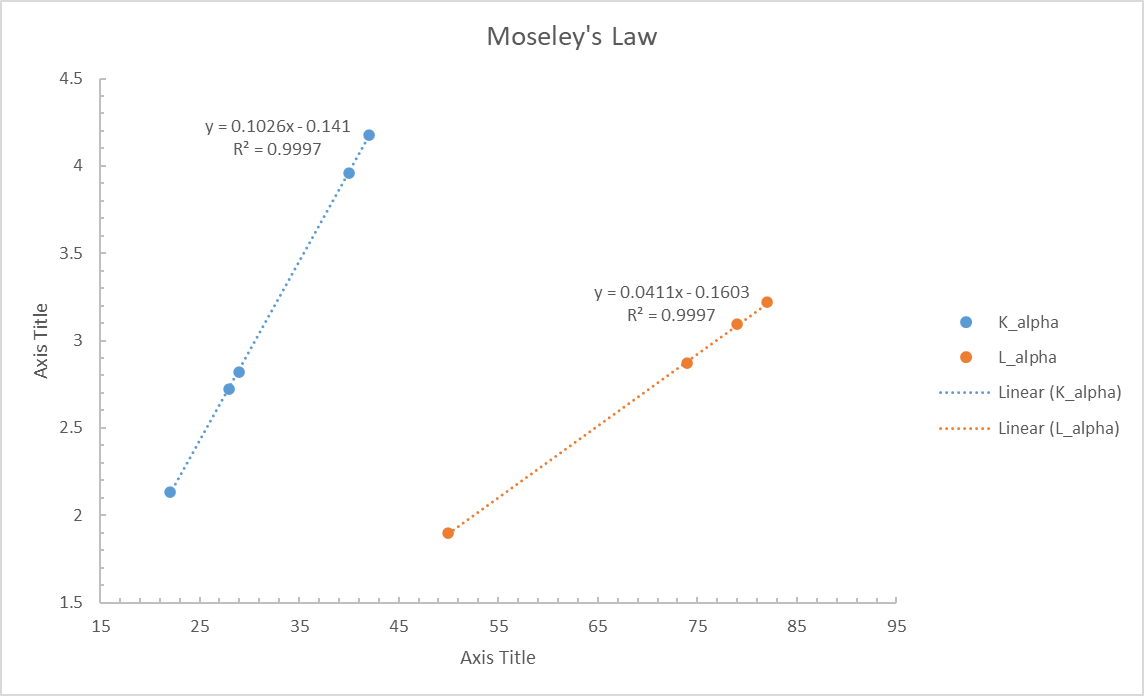
\includegraphics[width=0.7\textwidth]{img/moseleys.png}
    \caption{The figure shows a plot of $\sqrt{\varepsilon}$ vs $Z$ for given samples: \reminder{list samples}. The elements have been labelled on the plot. We have applied a linear fit to the two groups of data: (a) in blue, we have the samples for which we observe a \Kalpha line; (b) in orange, we have the samples for which we observe a \Lalpha line. The fit formula is also displayes next to the fitted line. \reminder{. produce better final figures}.}\label{fig:moseleys}
\end{figure}

Figure \ref{fig:moseleys} shows the fits for the two series. We can see that the data is fitted well by the model provided by Equation \eqref{eqn:moseleys-eqn}, given the experimental precision. We can therefore proceed to use X-ray K and L series lines as a signature of a given element in spectral analysis.

The ratio can also be calculated from the fitted values for the slopes, giving:
\begin{equation}
    \text{predicted: }\frac{m_\mathrm{K}}{m_\mathrm{L}} = \sqrt{\frac{27}{5}} = 2.324,\qquad \text{observed: } \frac{m_\mathrm{K}}{m_\mathrm{L}} = \frac{0.1026}{0.0411} = 2.496.
\end{equation}
Agreement is not so good, but we have not taken into account many other effects like change of energy due to being in a state $l \neq 0$ etc. So, not too bad. \reminder{must expand a bit maybe, + language style}.

\subsection{Provided alloys and semiconductors}
Now, can move to the analysis of samples. We will use fluorescence to determine the composition of the semiconductors from the non-MP part and of some unlabelled samples that are provided in the physics lab.

\subsubsection{Semiconductors}
The semiconductors are part of the non-MP experiment, where we determined their structure by determination of the lattice constant. Here, we provide an independent confirmation of our previous results. 
\begin{figure}[!htbp]
    \centering
    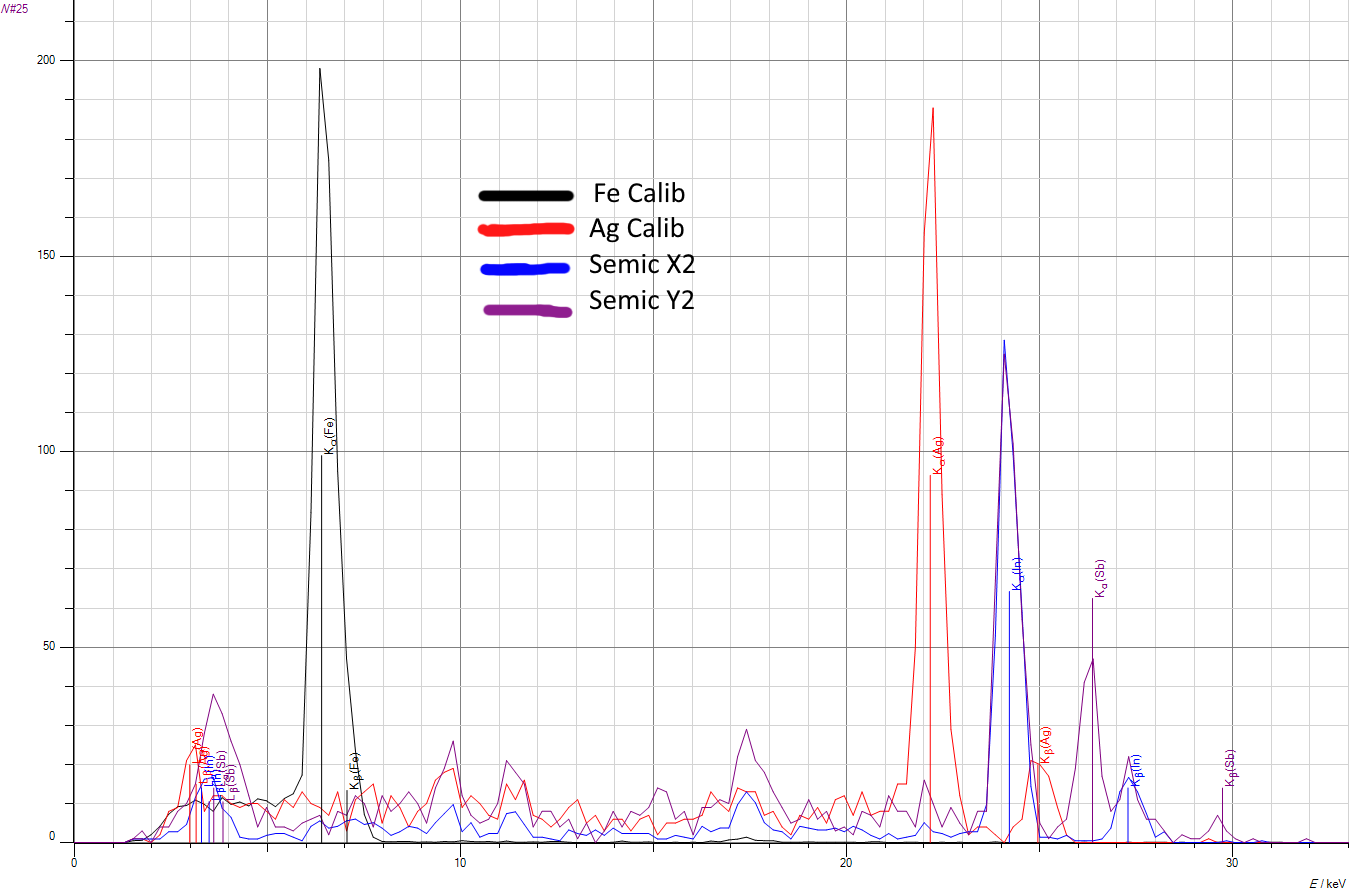
\includegraphics[width=0.7\textwidth]{img/spect-semiconductors.png}
    \caption{Fluorescence spectra of the Fe, Ag calibration and semiconductors labelled as X2 and Y2 in sample boxes provided. We see that X2 and Y2 show traces of In, and Y2 shows additionally traces of Sb. \reminder{prob should go to appendix?}}
    \label{fig:spect-semiconductors}
\end{figure}

We see that semiconductor Y2 shows traces of In and Sb, a group III and V elements respectively. This is a very common structure for semiconductors, so this is reassuring (\reminder{expand?}). In addition, this confirms our result from the first part of the practical, where we arrived at the conclusion that the semiconductor is an InSb via lattice diffraction. We can measure intensities of the \Kalpha lines for both, and calculate the ratios:
\begin{equation}
    \frac{n_\mathrm{In}}{n_\mathrm{Sb}} = \frac{I_\mathrm{In}}{I_\mathrm{Sb}} = \frac{122.5}{42.8} \approx 2.86 \quad \Rightarrow \quad p_\mathrm{In} = \frac{n_\mathrm{In}}{n_\mathrm{In}+n_\mathrm{Sb}} = 74 \% \quad p_\mathrm{Sb} = 26 \%
\end{equation}

For sample X2, we see a trace of In only. Checking with our result from the diffraction analysis, we see that the dopant is P (phosphorus). The characteristic X-rays of P in K-series (most energetic ones) have energies around \qty{2}{keV}, which is around our detection limit of about \qtyrange{2}{4}{keV}. This highlights one of the shortcomings of our method: it is limited in detecting only those elements, which have X-ray emission lines in the range of the bremsstrahlung and the range of operation of the detector.

\subsubsection{Unlabelled alloys}\label{subsubsec:unlabelled-alloys}
The lab has two boxes of unlabelled metallic samples - alloys of different metals. We can determine their composition and ratios by using Section \ref{subsec:compos-analysis}. Result is presented in Table \ref{tab:unlabelled-alloys}.

\begin{table}[htbp]
\centering
\sisetup{table-number-alignment=center, table-figures-integer = 1, round-mode = places}
\begin{tabular}{@{}
    lll
    S[table-figures-decimal = 2, round-precision=1]
    S[table-figures-decimal = 2, round-precision=2]
    S[table-figures-decimal = 2, round-precision=2]
    S[table-figures-decimal = 2, round-precision=2]
    S[table-figures-decimal = 2, round-precision=2]
    @{}
    }
\toprule
sample & element  & line   &{intensity}& {Kalph/Kbet}& {nA/nB}  & {prop}   & {by mass}   \\ \midrule
b1-1   & Cr       & Kalpha & 381.9     & 5.550872093 & 0.422877 & 0.297198 & 0.277555397 \\
b1-1   & Cr       & Kbeta  & 68.8      &             &          &          &             \\
b1-1   & Fe       & Kalpha & 903.1     & 4.138863428 &          & 0.702802 & 0.722444603 \\
b1-1   & Fe       & Kbeta  & 218.2     &             &          &          &             \\ \midrule
b1-2   & Cu       & Kalpha & 2110.2    & 6.136086072 & 1.783921 & 0.640794 & 0.691408371 \\
b1-2   & Cu       & Kbeta  & 343.9     &             &          &          &             \\
b1-2   & Zn       & Kalpha & 1182.9    & 17.09393064 &          & 0.359206 & 0.308591629 \\
b1-2   & Zn       & Kbeta  & 69.2      &             &          &          &             \\ \midrule
b1-3   & Cu       & Kalpha & 3947.9    & 14.32994555 & 1.265515 & 0.558599 & 0.613815022 \\
b1-3   & Cu       & Kbeta  & 275.5     &             &          &          &             \\
b1-3   & Zn       & Kalpha & 3119.6    & 16.51455797 &          & 0.441401 & 0.386184978 \\
b1-3   & Zn       & Kbeta  & 188.9     &             &          &          &             \\ \midrule
b2-a   & unusable &        &           &             &          &          &             \\ \midrule
b2-b   & unusable &        &           &             &          &          &             \\ \midrule
b2-c   & Fe       & Kalpha & 1351.9    & 3.736594804 & 2.062081 & 0.673425 & 0.694639809 \\
b2-c   & Fe       & Kbeta  & 361.8     &             &          &          &             \\
b2-c   & Zn       & Kalpha & 655.6     & 8.569934641 &          & 0.326575 & 0.305360191 \\
b2-c   & Zn       & Kbeta  & 76.5      &             &          &          &             \\ \midrule
b2-d   & Fe       & Kalpha & 1443.6    & 3.921760391 & 3.421664 & 0.773841 & 0.790561437 \\
b2-d   & Fe       & Kbeta  & 368.1     &             &          &          &             \\
b2-d   & Zn       & Kalpha & 421.9     & 9.743648961 &          & 0.226159 & 0.209438563 \\
b2-d   & Zn       & Kbeta  & 43.3      &             &          &          &             \\ \midrule
b2-e   & unusable &        &           &             &          &          &             \\ \midrule
b2-f   & Fe       & Kalpha & 1443.3    & 3.885060565 & 2.559496 & 0.719061 & 0.738463241 \\
b2-f   & Fe       & Kbeta  & 371.5     &             &          &          &             \\
b2-f   & Zn       & Kalpha & 563.9     & 9.367109635 &          & 0.280939 & 0.261536759 \\
b2-f   & Zn       & Kbeta  & 60.2      &             &          &          &             \\ \bottomrule
\end{tabular}
\caption{Table of the fitted intensities in alloy samples. Some of the measurements made had signal comparable with the background due to a human error during data acquisition; included here for completeness. \reminder{add a column with line energy, improve siunitx for number formatting, prob delete the unusable ones}}
\label{tab:unlabelled-alloys}
\end{table}

We can first check for consistency of the fits by looking at the rations of intensities for \Kalpha and \Kbeta, which should be approximately the same for al samples as it depends on the structure of the individual atom. Samples b2-c,d,f have close values for both the Fe and Zn lines. Since these two elements do not overlap in the spectrum (as seen in Figure \ref{fig:spect-b2-c}), these ratios should be close to the true ratio. We would expect to observe similar ratios in the other samples for Fe and Zn.

For sample b1-1, the Fe ratio is a little above 4, so we can say that the fit was pretty good. For samples b1-2,3, the Zn ratio is twice the one measured above. The fit here is pretty poor since Cu and Zn are respectively $Z=29$ and $Z=30$. Their spectra overlap by a lot (as seen in Fiugre \ref{fig:spect-b1-3}) --- the \Kalpha of Zn is between \Kalpha and \Kbeta of Cu. This, combined with the low resolution of our detector, makes it pretty difficult to fit here. Nevertheless, the \Kalpha lines are much stronger, so we can still try to extract the composition of the alloys.

Alloy composition is usually presented by mass in practical applications.These results are in the last column of Table \ref{tab:unlabelled-alloys}.

\subsection{International coins}
The lab has a box of various coins from around the world, the content of which we can again interpret using our fluorescence method, similar to the analysis in Section \ref{subsubsec:unlabelled-alloys}.

\begin{table}[!htbp]
    \centering
    \begin{tabular}{@{}lllllll@{}}
    \toprule
    No & Country        & Denomination   & Ni  & Cu  & Zn  & Other \\ \midrule
    3  & United Kingdom & 50p old        & yes & yes & no  & no    \\
    4  & United Kingdom & 50p new        & yes & yes & no  & no    \\
    5  & United Kingdom & 20p new        & yes & yes & no  & no    \\
    6  & United Kingdom & 10p old        & yes & yes & no  & no    \\
    7  & United Kingdom & 10p new        & yes & no  & no  & no    \\
    8  & United Kingdom & 2p new         & no  & yes & no  & no    \\
    9  & Singapore      & 1 dollar old   & yes & yes & no  & no    \\
    10 & Singapore      & 50c old        & yes & yes & no  & no    \\
    11 & Singapore      & 20c new        & yes & no  & no  & no    \\
    12 & Bulgaria       & 50 stotinki    & yes & yes & yes & no    \\
    13 & Bulgaria       & 5 stotinki     & no  & yes & no  & no    \\
    14 & European Union & 50c            & no  & yes & yes & no    \\
    15 & European Union & 2c old         & no  & yes & no  & no    \\
    16 & European Union & 2c new         & no  & yes & no  & no    \\
    17 & Romania        & 10 bani        & yes & no  & no  & no    \\
    18 & Norway         & 1 krone        & yes & yes & no  & no    \\
    19 & Switzerland    & 20 centim      & yes & yes & no  & no    \\
    20 & Sweden         & 1 krona        & yes & yes & no  & no    \\
    21 & Japan          & 1 yen          & no  & no  & no  & no    \\
    22 & Hong Kong      & 10c            & no  & yes & yes & no    \\
    23 & Uganda         & 200 schillings & yes & yes & no  & no    \\
    24 & USA            & 25c            & yes & yes & no  & no    \\
    25 & USA            & 1c             & no  & yes & yes & no    \\
    26 & Canada         & 25c            & yes & yes & no  & Fe?   \\
    27 & Brazil         & 5 centavos     & no  & yes & no  & no    \\ \bottomrule
    \end{tabular}
    \caption{Table of metal composition for a selection of international coins.}
    \label{tab:coin-measured}
\end{table}

When looking at plots of the spectra, we see that almost all coins are made predominantly out of Ni, Cu, and Zn with $Z=\numrange{28}{30}$ respectively. The spectra are overlapping, so similarly to the b1-2,3 samples in Section \ref{subsubsec:unlabelled-alloys}, we cannot really fit the samples well for all $\alpha, \beta$ lines. Nevertheless, we can still determine if one of the three elements is present. Additionally, we note down any additional features of the spectra that are of interest.The results can be summarised in Table \ref{tab:coin-measured}. Two exceptions to the general rule are obvious - the 1 Yen and 25c canadian coins. We can compare our results with the information from the institutions that issue these coins.

The official information lists the 1 Yen coin to be maid of 100\% aluminium (\reminder{citation needed}). The \Kalpha line for aluminum is at \qty{1.49}{keV}, out of the range of our setup. This is the reason we do not see any signal in our spectrum.

The official information informs us that the 25c canadian coin is a 94\% steel core with 6\% Ni-Cu plating (\reminder{citation needed}). When we look at the spectrum, however, the strength of the Fe line is much less than the Ni and Cu. This is due to the fact that the X-rays do not penetrate deep into the coin. If a thick enough coating is applied, we could even fully shield the steel core. In fact, several coins on our list follow this pattern, e.g. the new 2p and 10p coins.

\subsubsection{Why Ni,Cu,Zn?}
One obvious question that comes up form these results is why are alloys of Ni, Cu, and Zn the choice? There are several properties of these alloys that make them preferable for coin minting.

Historically, coins were most often made from gold, silver, and copper, with their value determined by the value of the metal in the coin. With the inflation of prices, however, the metal in the coins gradually became more expensive than their monetary value. There was a need for new materials to be implemented while keeping many of the familiar and useful properties of old coins.

Firstly, there are visual consideration of the coins. Ni-Cu and Cu-Zn alloys can have varying colours depending on the ratio of elements used. Ni-Cu are usually silver in appearance, while Cu-Zn alloys are usually golden in appearance, with small amounts of other additives sometimes present, like in the case of the \emph{nordic gold} alloy used for the make of the 50 euro cent coin.

Secondly, the cost considerations required some inexpensive materials to be used so that mass production is practical and coins are not produced at a loss. Due to inflation, this has also led to the change of coin composition throughout the years. One example is the UK 10p coin. While the old coin was made from pure Ni25Cu75, the new coin is made from 94\% steel clad in 6\% Ni. The method of implementing a cheaper core while using Ni,Cu,Zn for an outer layer also keeps the appearance the same or similar, which is one of the reasons for the approach.

Thirdly, the minting of the coins includes making the alloys and producing the coins with intricate detailing on their surfaces. The alloying of the specific ratios required by the specifications can be a difficult task outside of the specialised large scale industrial complexes. The three metals also allow for the detailing on different designs --- their alloys have been used to produce detailing by artisans for centuries (millennia?). Both of these specifics make the production of good counterfeit coins more difficult, which brings more security to the currency.

Finally, these alloys are very practical for everyday use. Coins, in their daily use, are exposed to the elements and physical wear. These alloys are very resistant to rusting (although Ni-Cu are often subject to formation of \emph{patina}) and have high durability against physical stresses like bending, stretching etc. This is another reason for the cladding method --- this gives them resistance against the elements and the physical toughness also helps preserve the detailing on the surface.
%sprinkle some citations pls.

\subsubsection{Cost-based analysis of coins.}
\reminder{This is a potential direction to investigate. Main idea --- calculate the ``value'' of a coin via its weight+official composition to see if anything interesting appears (coins worth more than their value, similar value for all coins etc.)}

\section{Conclusions}
In this experiment, we first study the theoretical basis of X-ray production first developed by Moseley. We measure the energy of the \Kalpha and \Lalpha emission lines series of several samples of known elements with known atomic number $Z=\numrange{22}{40}$ and $\numrange{50}{82}$, respectively. We find that there exists a linear relationship between the square root of the energy and number $Z$ as predicted by Moseley's law. Having established the uniqueness of X-ray emission lines for a given $Z$, we use it to study the composition of several samples by measuring their emission spectra when exposed to the continuous X-ray source. For the semiconductors, we observe traces of In in sample X2 and traces of In and Sb, which confirms the independently derived results form the non-mini-project \reminder{non-mini proj}. We also note the observational limitations of our setup, since the dopant of X2 was not observed --- P has a \Kalpha of energy below the observational limit.

Then, we study various metal alloys of unknown composition and the relative mass ratios of these samples. We measure these by performing Gaussian fits using the built-in capabilities of the acquisition software \reminder{fix}. We also go through some analysis to confirm our observations are self-consistent by comparing the ratios of \Kalpha to \Kbeta for the same elements in different samples.

Finally, we report on the composition of an array of international coins. We discover that most have signs of Ni,Cu, and Zn in their spectra, predominantly. While it is difficult to exactly extract intensities of the lines since they overlap, we report on the presence of either element in the coins in addition to any other element seen in the spectra. We discuss some seemingly anomalous results, like the 1 Yen and 25c canadian coins, which turn out to be 100\% aluminium and Ni-Cu clad steel. We conclude with an explanation for the frequency of use of these three metals, as well as the need to produce steel-core coins.

\reminder{future plans to improve: e.g. normalize with a plain bremsstrahlung to better fit values, esp if away from eachother.}

\bibliographystyle{plain}
% \renewcommand{\bibname}{#new-name} -- rename the title of bibliography chapter
\bibliography{references.bib}

\newpage
\appendix
\renewcommand\thesection{Appendix \Alph{section}}
\renewcommand{\thetable}{\Alph{section}\arabic{table}}
\setcounter{table}{0}
\renewcommand{\thefigure}{\Alph{section}\arabic{figure}}
\setcounter{figure}{0}
\renewcommand{\sectionmark}[1]{\markboth{\thesection.\ #1}{}}

\section{Energy spectra plots}
\begin{figure}[!htbp]
    \centering
    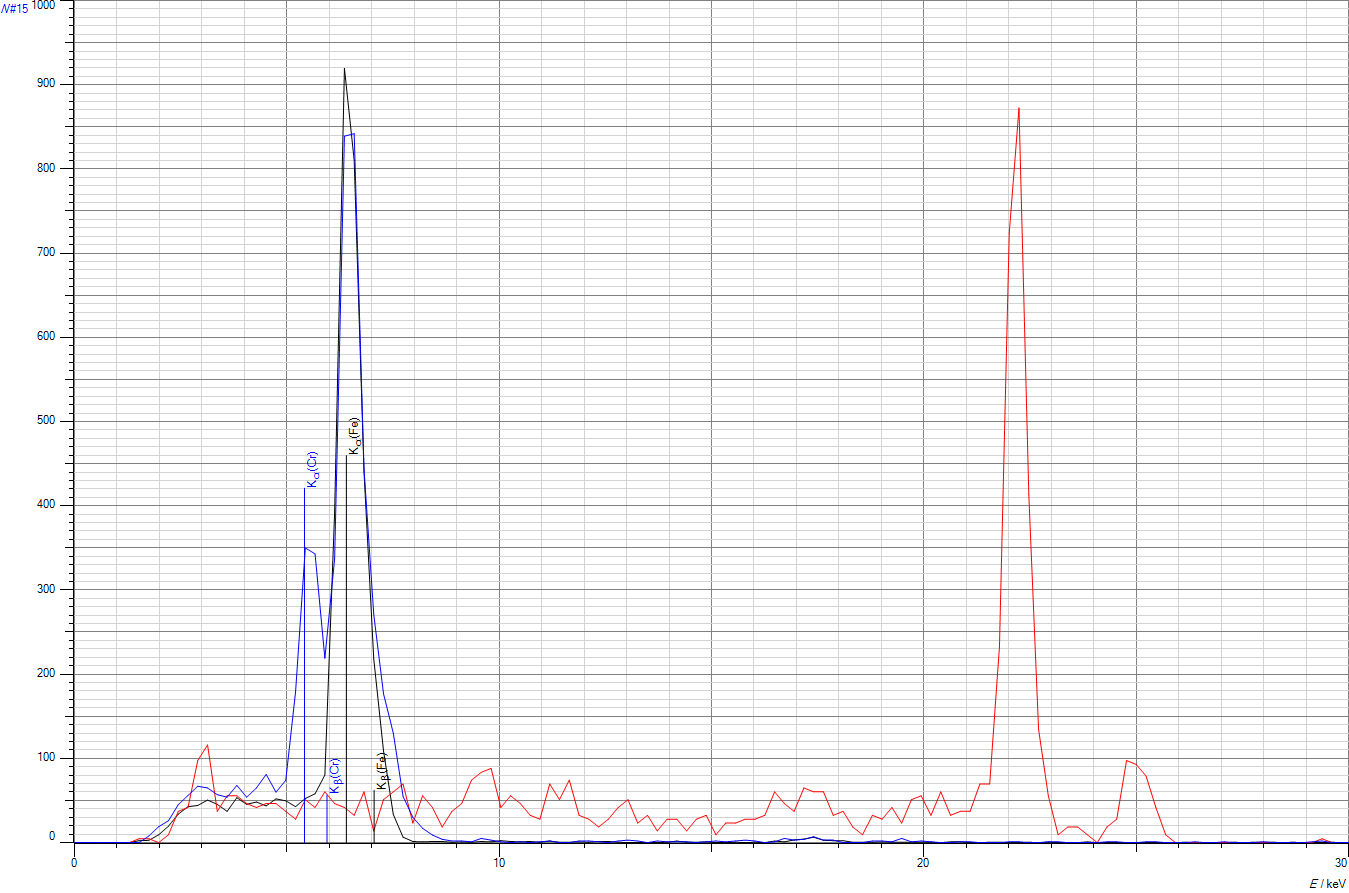
\includegraphics[width=0.7\textwidth]{img/spect-b1-1.png}
    \caption{Spectrum of sample b1-1. Calibration spectra of Fe and Ag in black and red respectively. It can be seen that the sample consists of Fe and Cr, and their spectra overlap. This presents a difficulty in fitting emission lines.}
    \label{fig:spect-b1-1}
\end{figure}
\begin{figure}[!htbp]
    \centering
    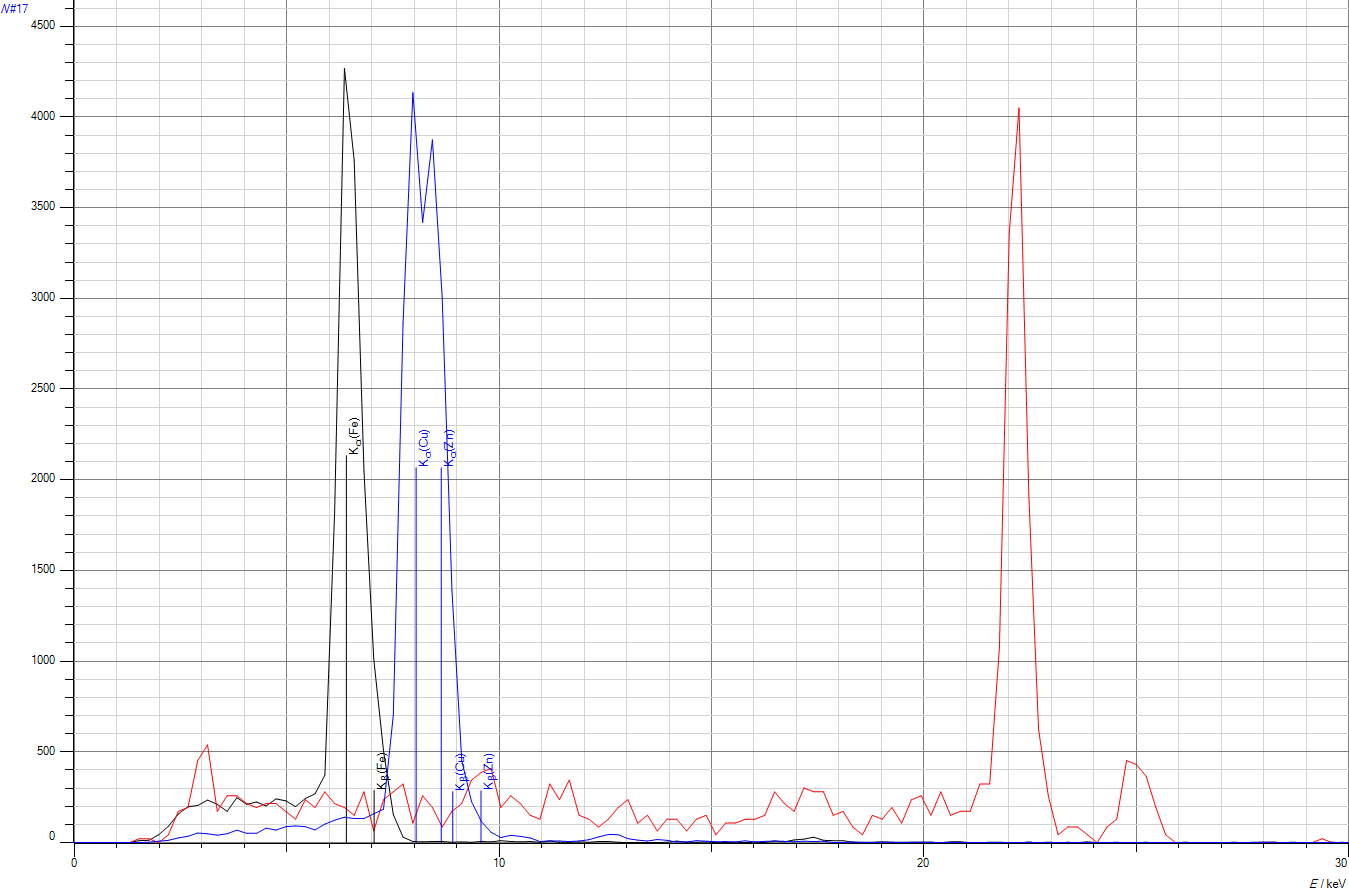
\includegraphics[width=0.7\textwidth]{img/spect-b1-3.png}
    \caption{Spectrum of sample b1-3. Calibration spectra of Fe and Ag in black and red respectively. It can be seen that the sample consists of Cu and Zn, and their spectra overlap significantly. This presents a difficulty in fitting emission lines.}
    \label{fig:spect-b1-3}
\end{figure}
\begin{figure}[!htbp]
    \centering
    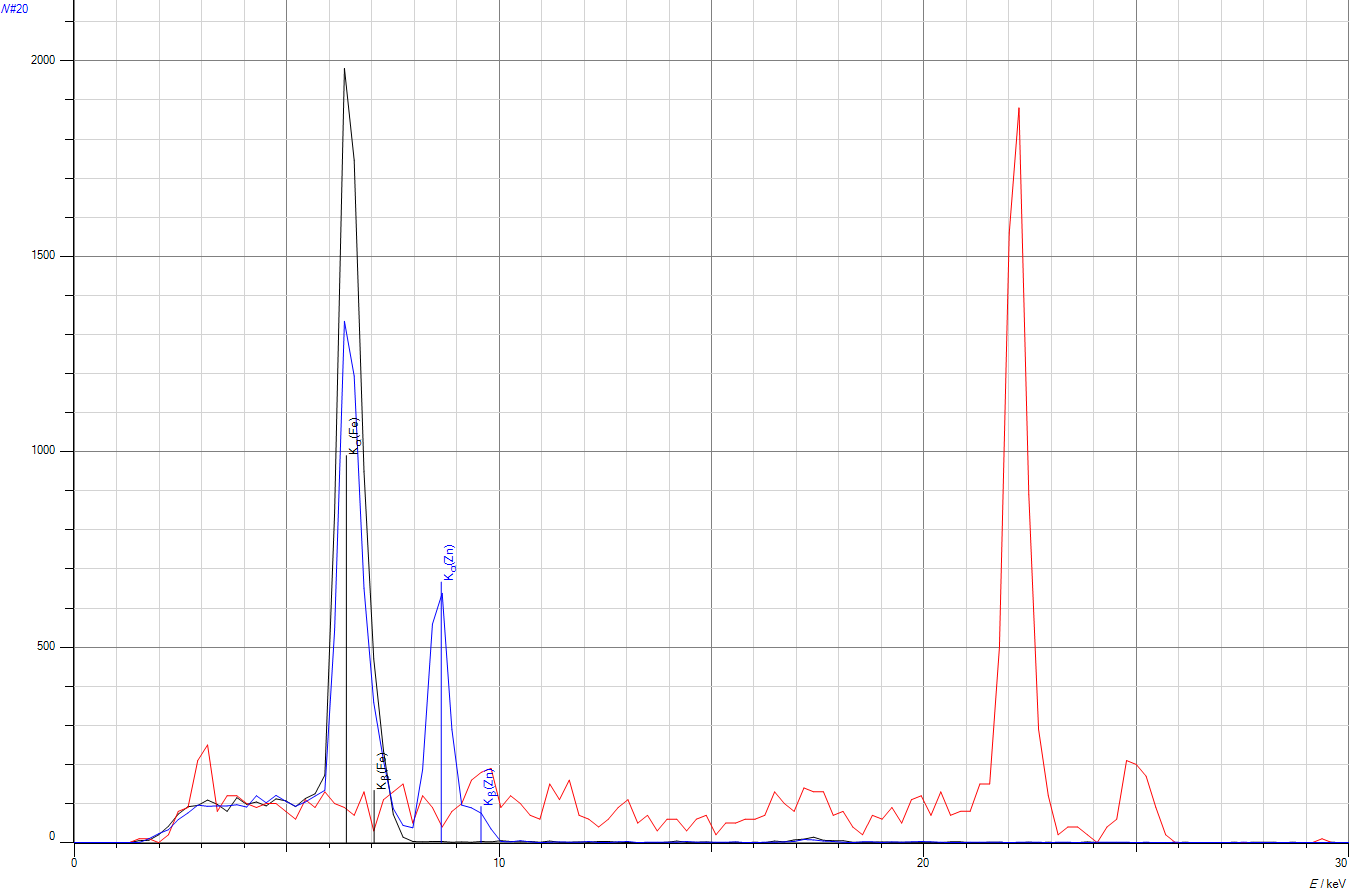
\includegraphics[width=0.7\textwidth]{img/spect-b2-c.png}
    \caption{Spectrum of sample b2-c. Calibration spectra of Fe and Ag in black and red respectively. It can be seen that the sample consists of Fe and Zn, and their spectra do not overlap.}
    \label{fig:spect-b2-c}
\end{figure}


\section{Extracted intensity data}
Add data here as tables, refer to it when needed.

\begin{table}[htbp]
    \centering
    \begin{tabular}{@{}llllllll@{}}
        \toprule
        No & Country        & Denomination   & Ni,\%    & Cu, \%   & Zn, \% & Other, \%            & Weight, g  \\ \midrule
        3  & United Kingdom & 50p old        & 25       & 75       & 0      & 0                    &            \\
        4  & United Kingdom & 50p new        & 25       & 75       & 0      & 0                    &            \\
        5  & United Kingdom & 20p new        & 16       & 84       & 0      & 0                    &            \\
        6  & United Kingdom & 10p old        & 25       & 75       & 0      & 0                    &            \\
        7  & United Kingdom & 10p new        & 6        & 0        & 0      & mild Steel - 94      &            \\
        8  & United Kingdom & 2p new         & 0        & 6        & 0      & mild Steel - 94      &            \\
        9  & Singapore      & 1 dollar old   & 2        & 92       & 0      & Al - 6               & 8.05+-0.20 \\
        10 & Singapore      & 50c old        & 25       & 75       & 0      & 0                    & 8.56+-0.20 \\
        11 & Singapore      & 20c new        & ?        & 0        & 0      & steel - ?            & 6.56+-0.28 \\
        12 & Bulgaria       & 50 stotinki    & 10       &          &        & 0                    & 5          \\
        13 & Bulgaria       & 5 stotinki     &          &          &        & steel - ?            & 3.5        \\
        14 & European Union & 50c            & 0        & 89       & 5      & Al - 5, Sn -1        & 7.8        \\
        15 & European Union & 2c old         &          & x        &        & 0                    & 3.06       \\
        16 & European Union & 2c new         &          & x        &        & 0                    & 3.06       \\
        17 & Romania        & 10 bani        & ?        & 0        & 0      & steel - ?            & 4          \\
        18 & Norway         & 1 krone        & 25       & 75       & 0      & 0                    & 4.35       \\
        19 & Switzerland    & 20 centim      & 25       & 75       & 0      & 0                    & 4          \\
        20 & Sweden         & 1 krona        & 25       & 75       & 0      & 0                    &            \\
        21 & Japan          & 1 yen          & 0        & 0        & 0      & al-100               & 1          \\
        22 & Hong Kong      & 10c            &          &          &        & 0                    & 1.85       \\
        23 & Uganda         & 200 schillings & $\sim$30 & $\sim$70 & 0      & 0                    & 8.5        \\
        24 & USA            & 25c            &          &          &        & 0                    &            \\
        25 & USA            & 1c             & 0        & 2.5      & 97.5   & 0                    & 2.5        \\
        26 & Canada         & 25c            & 2.2      & 3.8      & 0      & Steel AISI 1006 - 94 & 4.4        \\
        27 & Brazil         & 5 centavos     & 0        &          &        & 0                    &            \\ \bottomrule
    \end{tabular}
    \caption{Table of official info about the international coins. Notable are the coins with predominantly steel composition with a coating of one fo the three main elements. \reminder{CITATIONS}}
    \label{tab:coins-official}
\end{table}

\end{document}